\chapter{Background}

In the first part of the thesis we look at the current state of parsing techniques according to the literature. After that we provide a short overview of Elektra, the key-value storage framework we use in the thesis.

\section{State of the Art}
\label{sec:state_of_the_art}

The book \citetitle{grune2007parsing}~\cite{grune2007parsing} provides a good overview of various up-to-date parsing algorithms. It covers the most popular techniques (such as LL- and LR-Parsing~\cite{knuth1965translation}) and also less well known methods up to 2007. The book also describes various classification possibilities for parsing techniques \cite[p. 85]{grune2007parsing}. The most common classification is the division into bottom-up and top-down parsers.

\begin{figure}[H]
   \centering
   \subfloat[A top-down parser predicts and matches rules from the start symbol downwards.]{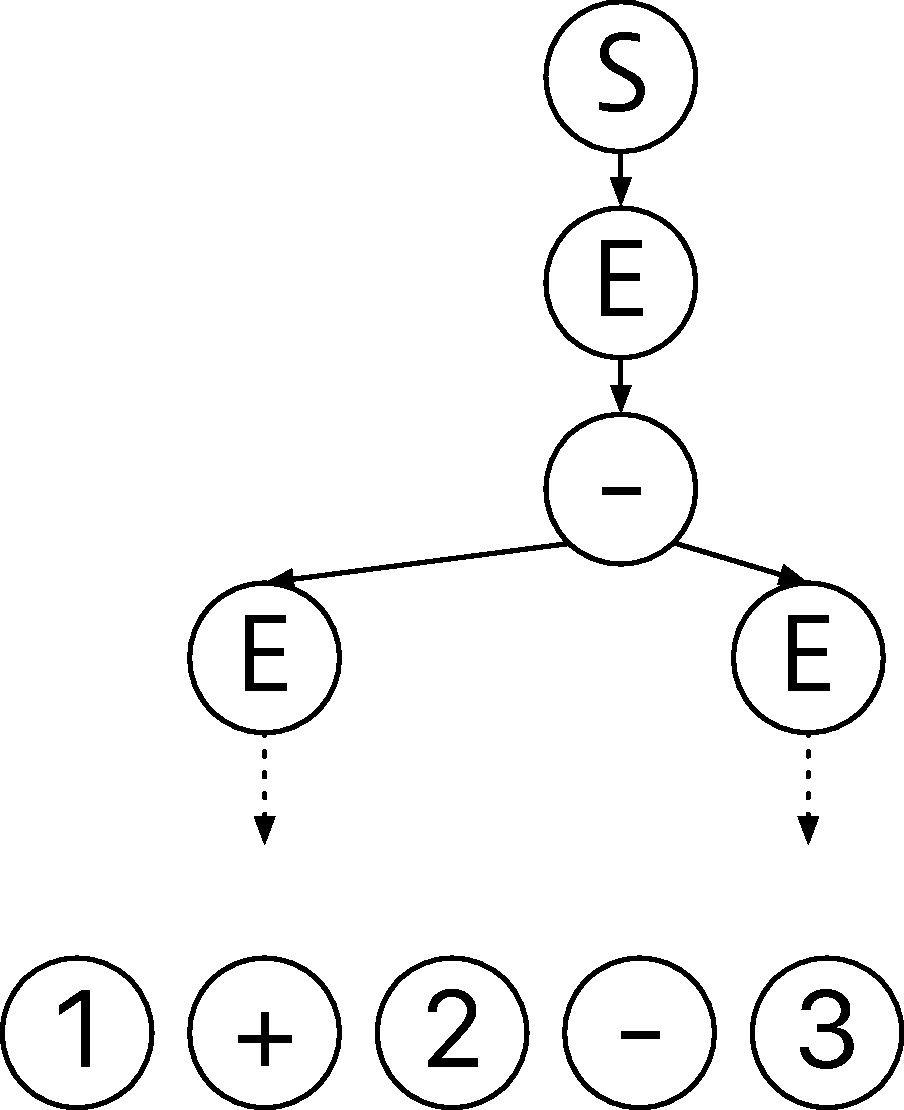
\includegraphics[width=.25\textwidth]{Top-Down}}
   \qquad
   \subfloat[A bottom-up parser recognizes text starting with the terminal symbols.]{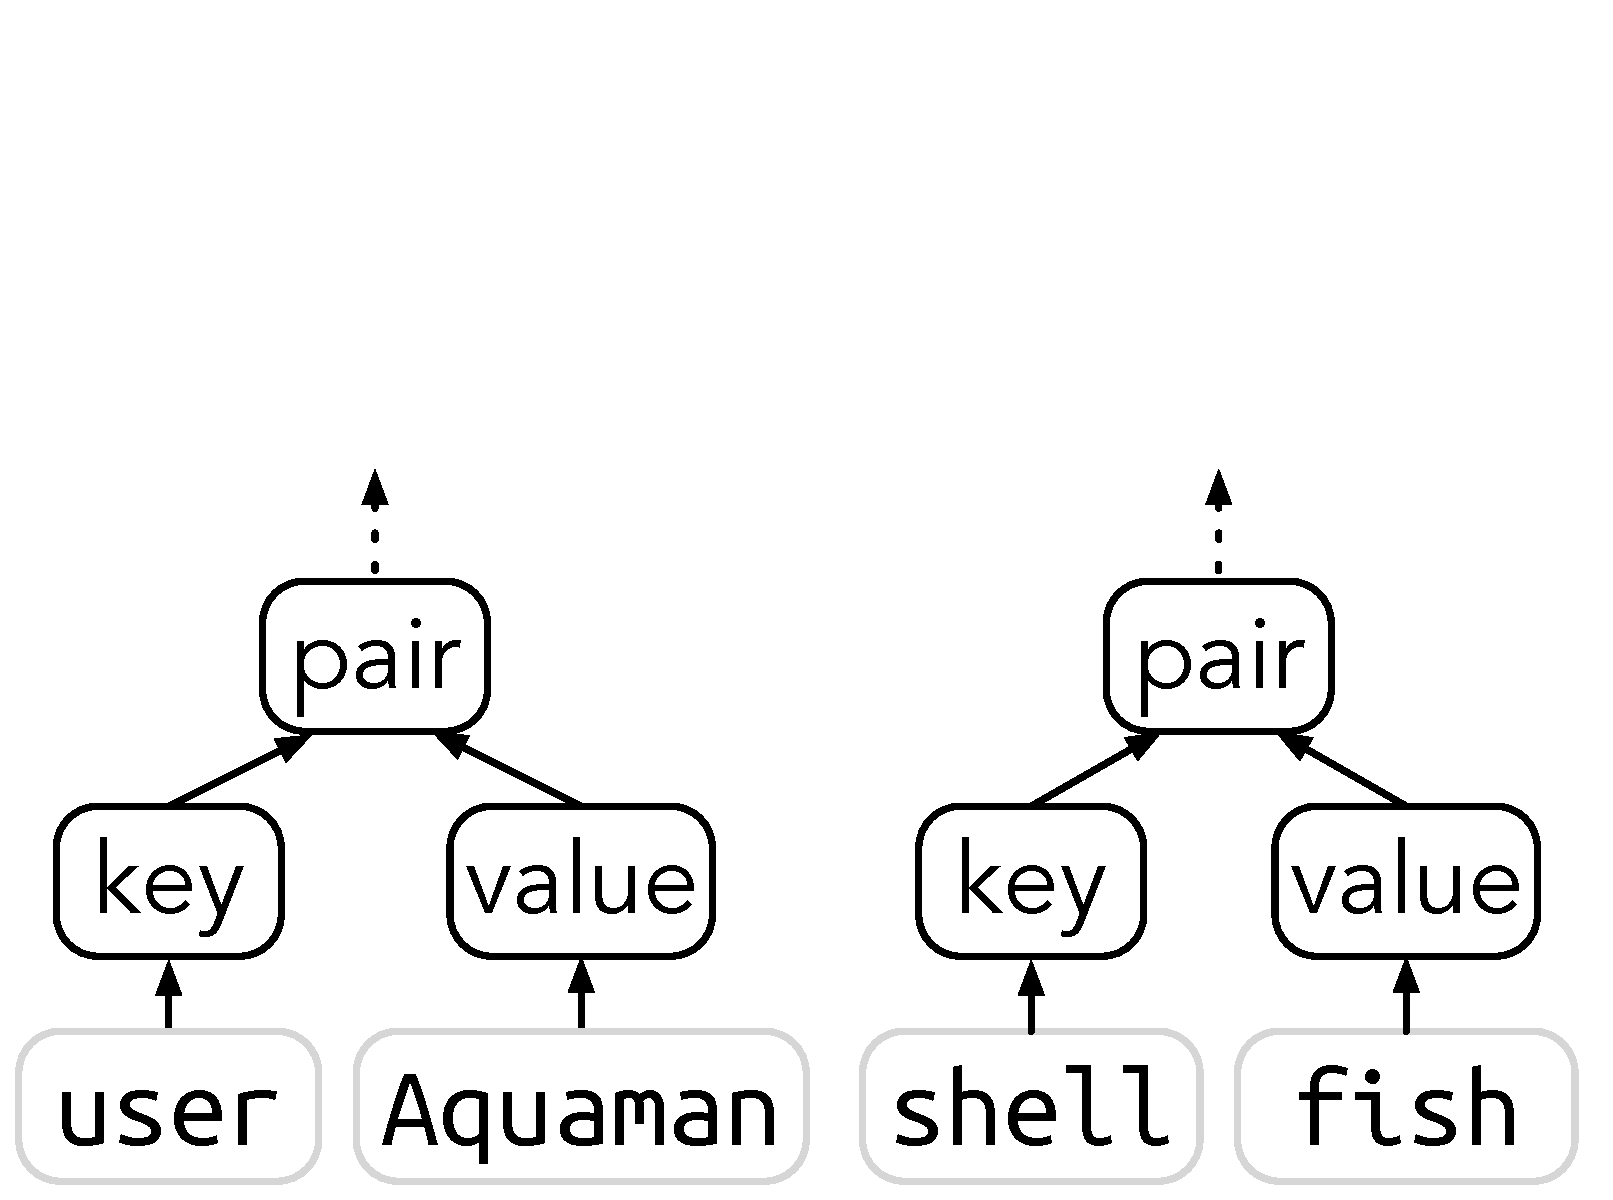
\includegraphics[width=.25\textwidth]{Bottom-Up}}
   \caption{Matching in top-down and bottom-up parsers}
 \end{figure}

In \emph{top-down parsing} the parser starts with a hypothesis about the structure of the given data. The parser then tries to predict and match parts of the structure, starting from larger parts working its way down-to smaller elements.

We can further categorize parsing into \emph{directional} and \emph{non-directional} methods. Directional methods read the input from left to right, while non-directional methods can use an arbitrary order. This implies that directional methods are simpler and faster, but less powerful, than their non-directional counterparts. As part of this thesis we only consider directional methods, since they are faster and powerful enough to parse configuration data.

One of the most popular directional top-down methods is \emph{LL parsing}. While this technique is quite old – \citetitle{grune2007parsing} (p. 584) mentions a paper from 1961 belonging to the LL category – it is still actively used and researched. The basic idea behind LL parsing is simple: Begin with the start symbol of the grammar and the first character of the text. Then predict the next grammar rule, looking at the text to the right of the current position. We can categorize the technique further depending on the number of characters/tokens the parser uses to predict the next rule. If the parser uses one token of look-ahead we speak of an LL(1) parser, if it uses k tokens of lookahead we speak of an LL(k) parser~\cite{rosenkrantz1969properties}.

Two common methods to create an LL parser are:

\begin{enumerate}

  \item Implement the parser code using a set of mutually recursive procedures (Recursive Descent Parser). The code for this is either written by hand or produced by a parser generator such as \GlsShort{ANTLR}~\cite{parr2013recursive}.

  \item Use a parser generator to create a table-based parser.

\end{enumerate}

Examples of popular active projects that use a handwritten recursive descent parser include \href{http://clang.llvm.org}{clang}~\cite{bendersky2012clang} and \href{http://gcc.gnu.org}{GCC}~\cite{myers2008cparser}. The \href{http://www.antlr.org/about.html}{about page} for \gls{ANTLR} mentions some projects that use its generated recursive descent parsers. The list includes Twitter, wich uses ANTLR for query parsing and parsers for the languages used in the Apache Hadoop projects Hive and Pig~\cite{parr2013definitive}.

Some of the latest research developments in LL-parsing include LL(*) parsing~\cite{parr2011ll} and its successor Adaptive LL(*)~\cite{parr2014adaptive} (ALL(*)). Both of these algorithms use dynamic lookahead~\cite[p. 1]{parr2011ll}. While LL(*) parsing uses a static algorithm for rule prediction, ALL(*) analyses the input at run-time to improve prediction. As consequence of this parsers using the ALL(*) algorithm will be faster after an initial warm-up phase~\cite[p. 3]{parr2014adaptive}. LL(*) is part of \gls{ANTLR}~3~\cite[p. 3]{parr2014adaptive}, while \gls{ANTLR}~4 uses Adaptive LL parsing.

As we already mentioned before, the other popular parsing technique besides top-down-parsing is \emph{bottom-up parsing}. In bottom-up parsing the parser builds a structure starting with the smallest elements of the grammar (terminals). The parser then combines these elements into larger parts. One of the earliest entries in the \emph{linear bottom-up} parser category is the LR(k) parser~\cite{knuth1965translation}. Just like in LL(k) parsing, k specifies the number of lookahead symbols the parser uses.

\begin{sloppypar}
Unlike LL parsers, LR parsers are usually not created by hand, but generated by a parsing tool such as \href{https://www.gnu.org/software/bison}{bison} or \href{http://dinosaur.compilertools.net/yacc}{yacc}. Since LR(k) tables are very large, even for a small numbers of k, the parser tools mentioned before generate less powerful but smaller and faster LALR(k)~\cite{deremer1969practical} parsers.
\end{sloppypar}

LR(k) parsers are able to handle more grammars, than LL(k) parsers for the same constant k~\cite[section “Lookahead”]{haberman2013ll}. However, LR parsers are still not able to use ambiguous grammars. For this purpose \citeauthor{lang1974deterministic} describes the Generalized LR (GLR)~\cite{lang1974deterministic} method that is also able to handle these types of grammars. GLR parser are sometimes also called Tomita parsers~\cite{tomita1985efficient} after the author that described the first implementation of a generalized LR parser.

Recent research in the space of directional bottom-up parsing includes improved versions of techniques that are almost as powerful as canonical LR(1). One of the most promising methods is IELR(1)~\cite{denny2008ielr}. The advantage of IELR(1) over LALR(1) is that it handles conflict resolution better. Parser tools such as bison use conflict resolution to handle non-LR grammars, i.e. grammars that contain rules where the parser is not able to decide what to do next. To handle these types of conflicts the grammar designer manually specifies which decision the parser should take. The current version of the parsing tool bison supports an experimental version of IELR(1).

Most parsing techniques can be categorized as either top-down or bottom-up. However, some techniques use a combination of both approaches. Others are usually not listed under one of the label top-down or bottom up, because they provide other features that the designer of these parsers deem more important, or they use features that do not fit well within either of these groups. In the remainder of this section we will discuss some of these techniques.

A method that can be categorized as either top-down technique with bottom-up recognition, or bottom-up technique with a top-down component~\cite[p. 206]{grune2007parsing} is \emph{Earley Parsing}~\cite{earley1970efficient}. Earley parsing is able to handle any context free grammar. This means the technique is as powerful as GLR parsing. This advantage comes at the cost of run-time. While LL parsing and LR parsing run in linear time depending on the length of the input ($O(n)$), Earley Parsing has an upper boundary of $O(n³)$. However, in \citeyear{leo1991general} \citeauthor{leo1991general} showed that an improved version of the algorithm handles most LR(k) grammars in linear time~\cite{kegler2011marpa, leo1991general, wikipedia2016Earley}. In \citeyear{aycock2002practical} \citeauthor{aycock2002practical} described improvements to the algorithm. Their version of Earley Parsing boosts the run-time in cases where the grammar contains nullable (empty) grammar rules. Recently \citeauthor{kegler2011marpa} incorporated the changes proposed by \citeauthor{leo1991general}, \citeauthor{aycock2002practical} in \href{http://savage.net.au/Marpa.html}{Marpa}~\cite{kegler2011marpa}.

\begin{figure}
  \centering
    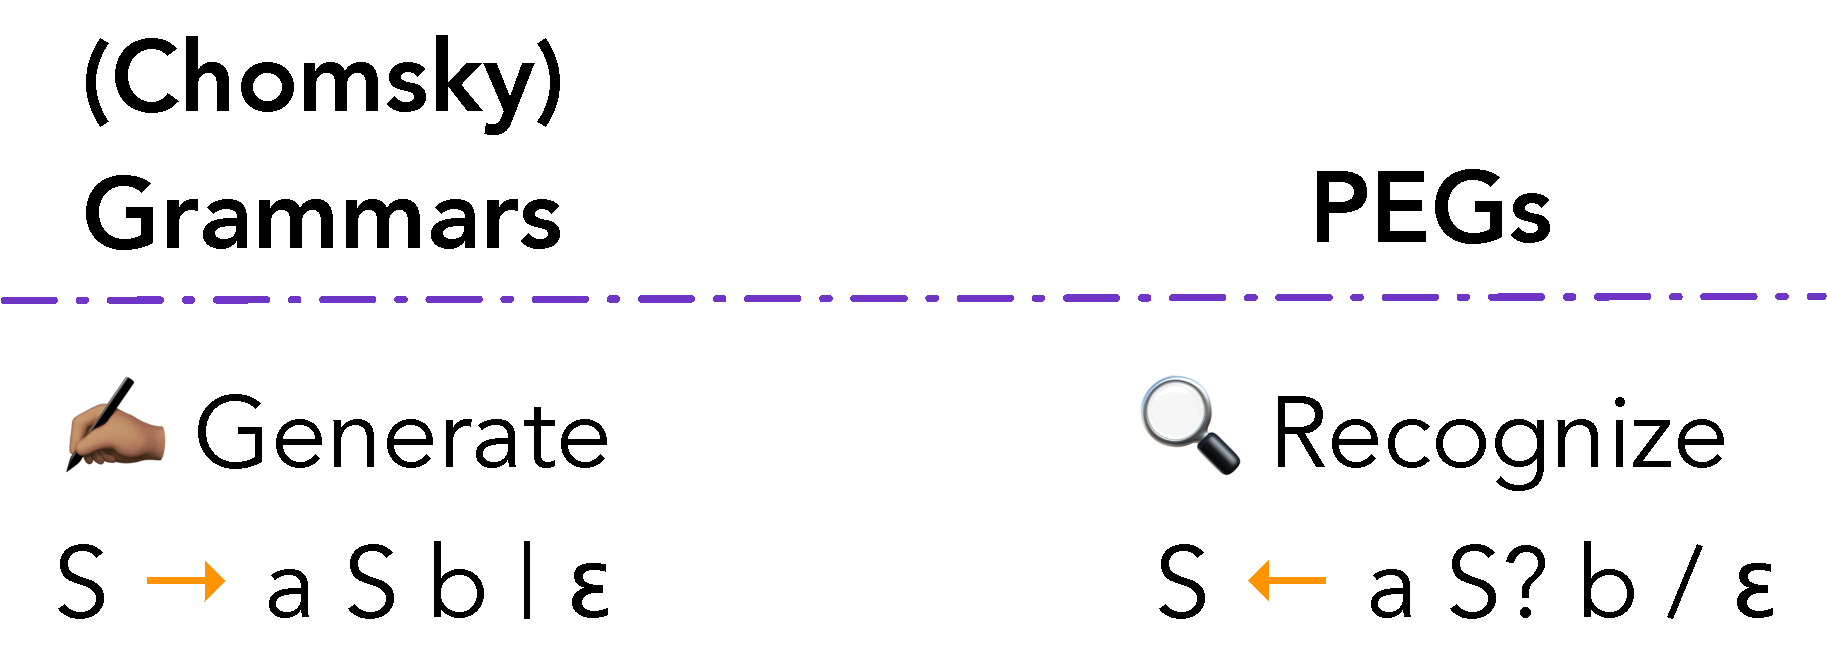
\includegraphics[width=0.45\textwidth]{Chomsky-PEGs}
  \caption{Both the Chomsky grammar on the left and the PEG on the right describe the same language $ \{ aⁿ bⁿ | n ≥ 0 \} $}
\end{figure}

All the methods we mentioned until now work with a description that is based on a (context-free) Chomsky grammar. These grammars describe a way to \emph{generate} words and sentences of a given language. Another way to specify the structure of a language is to give a description on how to \emph{recognize}~\cite[p. 506]{grune2007parsing} the words and sentences of a language. One popular recognition system are \glspl{PEG}. They were introduced by \citeauthor{ford2004parsing} in the paper \citetitle{ford2004parsing}~\cite{ford2004parsing}. \citeauthor{ford2002packrat} also describes how to write an efficient (top-down) parser that handles these types of grammars in linear time~\cite{ford2002packrat}. This method, called Packrat parsing, uses a specialized version of memoziation~\cite[p. 1]{ford2002packrat} to save intermediate results of the parsing process.

Just like Packrat parsing, \emph{combinatory parsing}~\cite{frost1992constructing, hutton1992higher} specifies a method to create recursive descent parsers. As the name suggests, the focus in combinatory parsing is the composability of parsers. The technique is usually used in functional programming languages, such as Haskell. These languages support higher order functions, i.e. functions that take other functions as their parameters~\cite[p. 564]{grune2007parsing}. In combinatory parsing the parser creator typically starts by specifying parsers (functions) for the simplest parts of the grammar (terminals). She or he then goes on to combine these simpler parsers into more powerful parsers for more complex rules (non-terminals). Combinatory parsing has similar problems as other top-down techniques such as LL parsing. One of these problems are left recursive grammar rules, i.e. rules that include references to themselves in the leftmost part of the right-hand side. Recently \citeauthor{frost2007modular} described a method to handle left recursive rules in combinatory parsing efficiently in the article \citetitle{frost2007modular}~\cite{frost2007modular}.

A method that is not a parsing technique per se, but a way to specify conversions of data from a source structure to a target structure and back is \emph{bidirectional programming}~\cite{foster2005combinators, bohannon2006relational}. The specification that allows this conversion is called a lens~\cite{foster2005combinators}.

\begin{figure}[H]
  \centering
    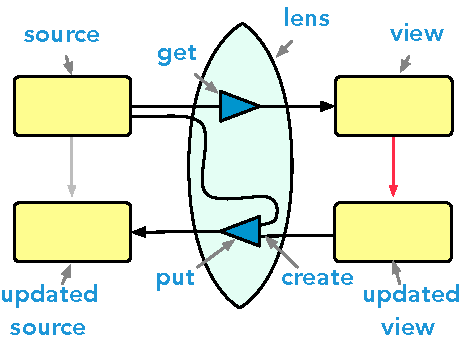
\includegraphics[width=.4\textwidth]{Lens.pdf}
  \caption{Lenses provide a way to both parse (get) and write (put) structured data \newline (Source: \href{http://www.seas.upenn.edu/~harmony/manual.pdf}{Boomerang Programmer’s Manual})}
\end{figure}

A programming language used to specify such lenses is Boomerang~\cite{bohannon2008boomerang}. The research of the Boomerang project lead to the creation of another project that uses lenses to parse configuration data: \href{http://augeas.net}{Augeas}. Augeas converts configuration data into a tree like representation. \citeauthor{berlakovich2016universal} implemented an Augeas plugin for Elektra as part of his Bachelor thesis~\cite{berlakovich2016universal}.

\section{Elektra}

\subsection{Keys and Key Sets}

In this section we describe some of the concepts of Elektra, the software that provides the common storage facility for our YAML parsers. Elektra is a framework that stores data in a \emph{global hierarchical key-value database}.

The most basic entity in Elektra is the \cc{Key} structure. A concrete instance of a \cc{Key} contains at least one non-empty attribute, which is the \emph{name} of the \cc{Key}. In the remainder of the thesis we will also often use the term \emph{key} - please notice the non-gray background – to refer to the name of a \cc{Key}.

\begin{figure}
  \centering
    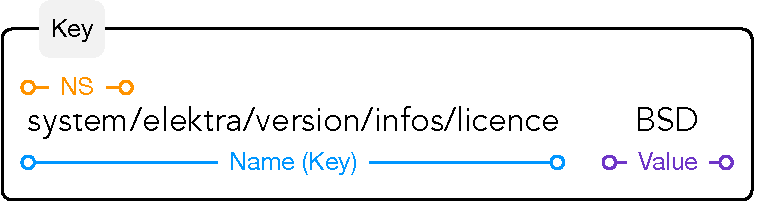
\includegraphics[width=.6\textwidth]{Figures/Key.pdf}
  \caption{In Elektra a \cc{Key} stores a single \textcolor{Aqua}{key}-\textcolor{Purple3}{value} pair. The first part of the name specifies the \textcolor{orange}{namespace} (NS).}
  \label{fig:Figures_Key}
\end{figure}

Besides the name an instance of a \cc{Key} usually also stores a value. Figure~\ref{fig:Figures_Key} shows an example \cc{Key} with the \textcolor{Aqua}{name} \code{system/elektra/version/infos/licence} and the \textcolor{Purple3}{value} \code{BSD}.

Since Elektra stores data in a hierarchical database, a key consists of parts – separated by \code{/} – that determine the location in the database. The key in Figure~\ref{fig:Figures_Key} consists of 5 parts. The first part \code{system} is the \textcolor{orange}{namespace} (NS) of the key. Elektra uses namespaces to specify context dependent data. For example, user specific data is stored under the namespace \code{user}. Elektra uses 5 namespaces to separate data:

\begin{itemize}[style=multiline, leftmargin=1.8cm]
  \item [\code{system}] specifies data values for the whole system,
  \item [\code{user}] contains data for the current user,
  \item [\code{dir}] stores data for the current directory,
  \item [\code{spec}] contains specification of other keys, and
  \item [\code{proc}] stores in memory data
\end{itemize}

. We can use a so-called \emph{cascading} key to select the most appropriate namespace. A cascading key does not start with a namespace but rather with a leading slash. Let us look at an example. If our database contains the keys:

\begin{itemize}
  \item \code{system/key}
  \item \code{user/key}
\end{itemize}

, then Elektra will select the key \code{user/key} if we use the cascading key \code{/key} to retrieve data. If the database also contains a key \code{dir/key} for the current working directory, then Elektra will select this key instead.

As we already saw in the example above usually we store not only one, but multiple key-value pairs in the database. For this purpose Elektra provides the structure \cc{KeySet}. A \cc{KeySet} contains a set of \cc{Key} objects, where the name of each \cc{Key} has to be different. If we add a new entry with an already existing name to the \cc{KeySet}, then Elektra will just overwrite the old \cc{Key} with the same name.

\begin{figure}
  \centering
    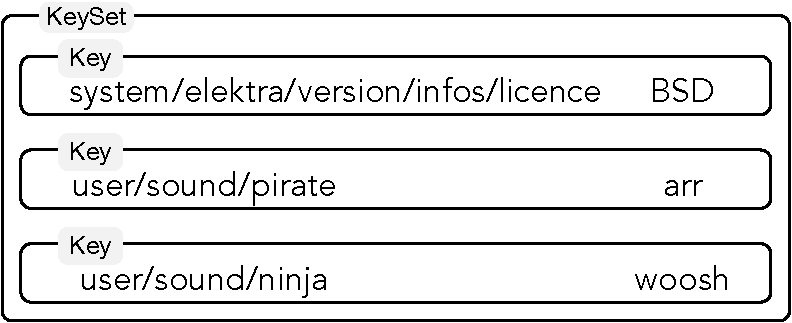
\includegraphics[width=.6\textwidth]{Figures/KeySet.pdf}
  \caption{Elektra uses \cc{KeySet} structures to save multiple key-value pairs}
  \label{fig:Figures_KeySet}
\end{figure}

Elektra also uses the \cc{KeySet} structure to add \emph{metadata} to single keys. For this purpose each \cc{Key} may store a \cc{KeySet} containing simple key-value pairs. Figure~\ref{fig:Figures_Metadata} shows an example \cc{Key} containing two meta keys \code{comment} and \code{check/type}.

\begin{figure}
  \centering
    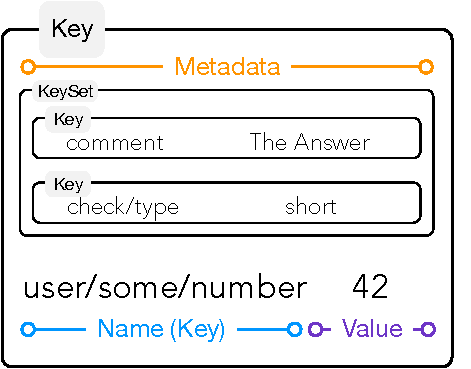
\includegraphics[width=.4\textwidth]{Figures/Metadata.pdf}
  \caption{Elektra uses a \cc{KeySet} to save metadata for a \cc{Key}}
  \label{fig:Figures_Metadata}
\end{figure}

\FloatBarrier
\subsection{Plugins}

Apart from basic features most of Elektra’s functionality is realized as \emph{plugin}. This has the advantage, that Elektra’s core can stay minimal only requiring \href{https://en.wikipedia.org/wiki/C99}{C99}, while plugins are able to implement and use OS specific features.

There are many different plugin categories, but the most basic ones are resolver and storage plugins. Elektra needs at least one resolver and one storage plugin. The resolver plugin is responsible for resolving filenames and replacing files on disk. Storage plugins on the other hand parse configuration files and convert read data to a \cc{KeySet}. They are also responsible for writing a modified \cc{KeySet} back to a given file.

In this thesis we are mostly interested in storage plugins. However, we will also use other plugins to implement common functionality for our YAML storage plugins. For this purpose we use the plugin interface of Elektra to pass key sets between plugins.

The order in which Elektra calls a certain plugin is specified via the \emph{contract} of the plugin. For example, a typical storage plugin will use the positions \code{getstorage} and \code{setstorage}. Plugins at the position \code{getstorage} will be called when Elektra tries to read a configuration file, while Elektra calls \code{setstorage} plugins when it is time to write a \cc{KeySet} back to a file. A plugin that wants to further process data will usually use the position \code{postgetstorage} right after \code{getstorage}, and \code{presetstorage} the position before \code{setstorage}.

\begin{figure}
  \centering
    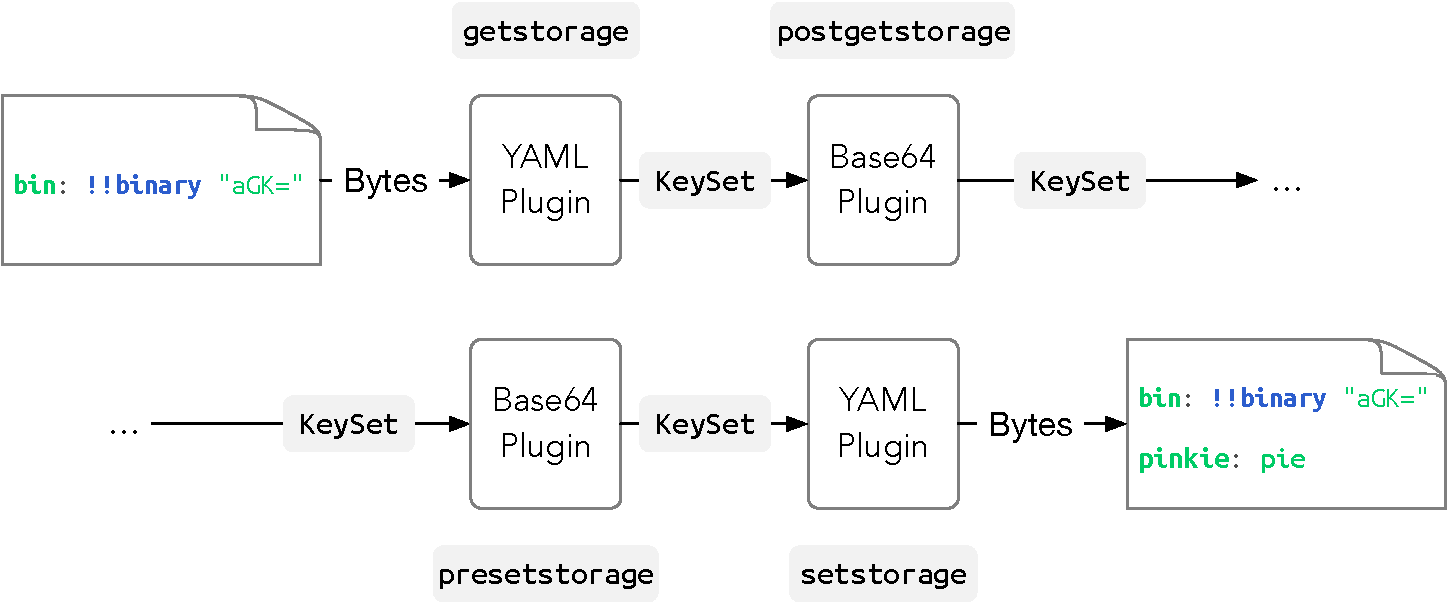
\includegraphics[width=.9\textwidth]{Figures/Plugins.pdf}
  \caption{Elektra uses multiple plugins to process data}
  \label{fig:Figures_Plugins}
\end{figure}

Figure~\ref{fig:Figures_Plugins} shows a example, where Elektra uses a YAML plugin to read and write data, while a Base64 plugin (see also section “\nameref{sec:base64}”) encodes and decodes binary values. Such a combination of multiple plugins working together is called a \emph{backend}.

In Elektra we \emph{mount} a backend at a certain position of the key-value database. For example, if we mount the backend described above at \code{user/yaml}, then the YAML plugin is responsible for storing and retrieving values below this mountpoint. If we want to save a new \cc{Key} with the name \code{user/yaml/pinky} and the value \code{pie}, then Elektra

\begin{enumerate}
  \item uses the YAML plugin to convert the current YAML configuration file to a \cc{KeySet},
  \item decodes every binary \cc{Key} with the Base64 plugin,
  \item adds \code{user/yaml/pinky} to the \cc{KeySet},
  \item encoded every binary \cc{Key} with the Base64 plugin, and
  \item then stores the result to the configuration file using the YAML plugin
\end{enumerate}

.
